
\documentclass[10pt]{beamer}
\usepackage{epstopdf}
\usepackage{amsmath,amsthm,amsfonts}
\usepackage{tikz,pgfplots}
\usepackage{animate}
\usepackage{graphicx}
%\usepackage[margin=1.75cm]{geometry}
\usepackage{setspace}
%\onehalfspacing
%\allowdisplaybreaks
%\usepackage[colorlinks]{hyperref}

\newcommand\abs[1]{\left|#1\right|}


% ============================================================
% You must have the following files in your working directory:
% beamerthemeCarroll.sty and CarrollLogo.pdf 
% ============================================================
\usetheme{Carroll} % this tells beamer to use the Carroll College theme 

\usepackage{amsmath,amsthm,graphicx,tikz,pgfplots} % some basic packages 


% ============================================================
% insert your information for the presentation
% ============================================================
\author{Presented by: Jordan Trinka\\ Advisor: Eric Sullivan, Ph.D.}
\title[Short Title]{ Modeling Contaminant Flow in the \\Puget Sound}
\subtitle{A Finite Element Implementation of the Advection-Diffusion Equation} % A subtitle is optional. Delete or comment this line if not used
\date{April 8, 2017} % Insert date of presentation


% ========================= NOTES ============================
% If you use sections and subsections then these will appear on 
% the header bar at the top of the slide. If you do not use 
% sections and subsections then the frame title will appear
% on the header bar.
%
% The color theme is chosen to best match the branding standards
% of Carroll College. 
% 
% If there are questions about using this theme please contact
% Eric Sullivan at esullivan@carroll.edu
% ============================================================


\begin{document}

% ============================================================
% The following is the title page. The [t,plain] command 
% ensures that the title page has the proper formatting
% ============================================================
\begin{frame}[t,plain]
    \titlepage
\end{frame}

% ============================================================
% start the content of the presentation
% ============================================================
%\begin{frame}{Contents}
%\frametitle{Contents}
    %\tableofcontents[
%]
%\end{frame}

\section{Introduction}

\begin{frame}{Purpose} \label{Purpose}
\begin{itemize}
\item Deepwater Horizon spill of April, 2010
\item Predictive analysis
\item Clean up cost
\item Clean up time
\item Environmental Protection
\end{itemize}

 \includegraphics[width=0.4\linewidth]{deepwater.jpg}
\tiny
\\
http://www.greenpeace.org/international/en/multimedia/photos/Deepwater-Horizon---Wellhead/
\normalsize
\\
\hyperlink{Questions}{\beamergotobutton{Questions}}
\end{frame}

\begin{frame}{Overview}\label{Overview}

\begin{itemize}
\item Model contaminant flow in a two-dimensional model of the Puget Sound
\item Advection-Diffusion Equation
\item Navier-Stokes Equation
\end{itemize}

\end{frame}


\begin{frame}{Puget Sound Domain}\label{Puget Sound Domain}
\begin{figure}

   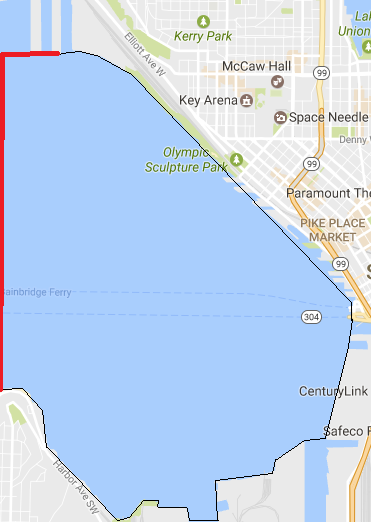
\includegraphics[width=0.4\linewidth]{domainoutline.png}
\end{figure}
\hyperlink{Questions}{\beamergotobutton{Questions}}
\end{frame}

\begin{frame}{Puget Sound Domain Triangularization}\label{Puget Sound Domain Triangularization}
\begin{figure}

   \includegraphics[width=0.5\linewidth]{mathpointani_img_1.png}
\end{figure}
\hyperlink{Questions}{\beamergotobutton{Questions}}
\end{frame}


\section{The Advection-Diffusion Equation, Discretization, and Weak Form} 
\begin{frame}{The Advection-Diffusion Equation}\label{The Advection-Diffusion Equation}
\begin{equation}
\frac{\partial u}{\partial t}= D\Delta u + \underline{v} \cdot \underline{\nabla}u+f
\end{equation}
\begin{itemize}
\item $u \in  H^{1}\left(\Omega \right)$
\item $\frac{\partial u}{\partial t} \rightarrow$ Change in concentration with respect to time
\item $\Delta u \rightarrow$ Diffusivity term
\item $D \rightarrow$ Coefficient of diffusion
\item$\underline{v} \cdot \underline{\nabla}u \rightarrow$ Advective term
\item $f \in L^{2}\left(\Omega \right)\rightarrow$ Forcing function 
\end{itemize}
\hyperlink{Questions}{\beamergotobutton{Questions}}
\end{frame}


\begin{frame}{Implict Euler Step and the Weak Form}  \label{EulerandWeak}
\begin{equation}
\frac{\partial u}{\partial t}= D\Delta u + \underline{v} \cdot \underline{\nabla}u+f
\end{equation}
\begin{itemize}
\item Implicit in time Euler Step
\end{itemize}
\footnotesize
\begin{equation}
U^{n}-dtD\Delta U^{n}-dt\underline{v}\cdot \underline{\nabla}U^{n}=U^{n-1}.
\end{equation}
\normalsize
\begin{itemize}
\item Derive the Weak Form
\end{itemize}
\footnotesize
\begin{equation}
\int_{\Omega}U^{n}W dx -dtD\alert{ \int_{\Omega}\Delta U^{n}W dx}-dt\int_{\Omega}\left(\underline{v}\cdot \underline{\nabla}U^{n}\right)W dx=\int_{\Omega} U^{n-1}W dx
\end{equation}

\begin{itemize}
\item $W \in H^{1}\left({\Omega}\right)$
\item $\Omega \rightarrow$ Domain
\end{itemize}

\begin{equation}
\int_{\Omega}U^{n}W dx +dtD\int_{\Omega}\underline{\nabla}W \cdot \underline{\nabla} U^{n} dx-dt\int_{\Omega}\left(\underline{v}\cdot \underline{\nabla}U^{n}\right)W dx=dtD\int_{\Gamma_{N}}g^{n}W ds+ \int_{\Omega} U^{n-1}W dx.
\end{equation}
\normalsize

\hyperlink{Questions}{\beamergotobutton{Questions}}
\end{frame}


\section{Application of the Finite Element Method}
\begin{frame}{Creation of Basis Functions and Finite Element Discretization} \label{basisfunctionandfinite}
\begin{itemize}
\item Define the following
\end{itemize}
$$
\eta_{k}\left(x_{i},y_{j}\right)=\begin{cases}
1 \texttt{ if } i,j=k\\
0 \texttt{ if } i,j \neq k \texttt{ for } i,j,k=1,...,N
\end{cases} 
$$

\begin{itemize}
\item Express $U^{n}$ and $W$ as a linear combinations of basis functions
\end{itemize}

\begin{eqnarray}\label{UWdiscrete}
U^{n}\left(x,y\right)&=&\sum_{i=1}^{N}\xi_{i}\eta_{i}\left(x,y\right), \texttt{ } x,y \in \Omega \\
\nonumber
W\left(x,y\right)&=&\sum_{j=1}^{N}\beta_{j}\eta_{j}\left(x,y\right), \texttt{ } x,y \in \Omega
\end{eqnarray}

\begin{itemize}
\item $\xi_{i}=U^{n}\left(x_{i},y_{i}\right)$
\item $\beta_{j}=W\left(x_{j},y_{j}\right)$
\end{itemize}

\hyperlink{Questions}{\beamergotobutton{Questions}}
\end{frame}

\begin{frame}{Applying the Finite Element Discretizations to the Weak Form} \label{applyingFEMtoweakform}
\footnotesize
\begin{equation}
\int_{\Omega}U^{n}W dx +dtD\alert{\int_{\Omega}\underline{\nabla}W \cdot \underline{\nabla} U^{n} dx}-dt\int_{\Omega}\left(\underline{v}\cdot \underline{\nabla}U^{n}\right)W dx=dtD\int_{\Gamma_{N}}g^{n}W ds+ \int_{\Omega} U^{n-1}W dx.
\end{equation}
\normalsize

\begin{itemize}
\item  Substitute in linear combination discretizations for $\underline{\nabla}W$ and $\underline{\nabla}U^{n}$
\end{itemize}

\begin{equation}
\sum_{i=1}^{N}\sum_{j=1}^{N} \int_{\Omega} \underline{\nabla}\eta_{j} \xi_{j} \cdot \underline{\nabla}\eta_{i} \beta_{i} dx
\end{equation}


\begin{itemize}
\item Sum all the contributions from each of the different triangular elements that form each basis function
\end{itemize}

\begin{equation}
 \xi_{j}\beta_{i}\sum_{T \in T_{\Omega}}\int_{T} \underline{\nabla} \eta_{j} \cdot \underline{\nabla}\eta_{i} dx, \texttt{ } i,j=1,...,N
\end{equation}

\hyperlink{Questions}{\beamergotobutton{Questions}}
\end{frame}

\begin{frame}{Building the Linear System}\label{BuildLinearSystem}

\begin{equation}
\xi_{j}\beta_{i}\alert{\sum_{T \in T_{\Omega}}\int_{T} \underline{\nabla} \eta_{j} \cdot \underline{\nabla}\eta_{i} dx}, \texttt{ } i,j=1,...,N
\end{equation}

\begin{itemize}
\item Define $\mathbf{A} = \sum_{T \in T_{\Omega}}\int_{T} \underline{\nabla} \eta_{j} \cdot \underline{\nabla}\eta_{i} dx$
\end{itemize}

\begin{itemize}
\item Apply similar techniques on the rest of the weak form
\end{itemize}

\footnotesize
\begin{equation}
\underbrace{\int_{\Omega}U^{n}W dx}_{ \xi_{j}\beta_{i}\mathbf{B}} +dtD\underbrace{\int_{\Omega}\underline{\nabla}W \cdot \underline{\nabla} U^{n} dx}_{ \xi_{j}\beta_{i}\mathbf{A}}-dt\underbrace{\int_{\Omega}\left(\underline{v}\cdot \underline{\nabla}U^{n}\right)W dx}_{ \xi_{j}\beta_{i}\mathbf{C}}=dtD\underbrace{\int_{\Gamma_{N}}g^{n}W ds+ \int_{\Omega} U^{n-1}W dx}_{ \beta_{i}\underline{b}}.
\end{equation}

\normalsize
for $i,j=1,...,N$
\hyperlink{Questions}{\beamergotobutton{Questions}}
\end{frame}

\begin{frame}{ Mass Matrices, Right-Hand Side, and the Linear System} \label{MassmatRHSLinearSystem}
\begin{itemize}
\item The expressions for $\mathbf{B}$, $\mathbf{C}$, and $\underline{b}$  (Alberty, Carstensen, Funken)
\end{itemize}

\begin{equation}
\mathbf{B}_{i,j} = \sum_{T \in T_{\Omega}} \int_{T} \eta_{j}\eta_{i} dx.
\end{equation}

\begin{equation}
\mathbf{C}_{i,j} = \sum_{T \in T_{\Omega}}\int_{T}\left(\underline{v}\cdot \underline{\nabla}\eta_{j}\right)\eta_{i} dx.
\end{equation}

\begin{equation}
\underline{b}_{i}= \sum_{E \in \Gamma_{N}} Ddt\int_{E}g^{n}\eta_{j}ds+\mathbf{B}\xi_{j}^{n-1}
\end{equation}
 $i,j=1,...,N$
\begin{itemize}
\item $\xi_{j}^{n-1} = U^{n-1}\left(x_{j},y_{j}\right)$
\item $E \rightarrow$ edge on $\Gamma_{N}$
\end{itemize}
\begin{equation}
\left(\mathbf{B}+dtD\mathbf{A}-dt\mathbf{C}\right)\underline{\xi}^{n}=\underline{b}^{n}.
\end{equation}
\hyperlink{Questions}{\beamergotobutton{Questions}}
\end{frame}

\begin{frame} {Computation of $\mathbf{C}$} \label{ComputationofC}

Computational techniques used for $\mathbf{A}$, $\mathbf{B}$, and $\underline{b}$ are covered in Alberty, Carstensen, and Funken
\begin{itemize}
\item Compute $\mathbf{C}$ by first realizing $\underline{v} \cdot \underline{\nabla}\eta_{j}$ is a constant
\end{itemize}
\begin{equation}
\mathbf{C}_{i,j} = \underline{v}\cdot \underline{\nabla}\eta_{j}\sum_{T \in T_{\Omega}}\int_{T}\eta_{i} dx.
\end{equation}

\begin{itemize}
\item Barycentric approximation of the basis functions when $N$ is large
\end{itemize}

\begin{equation}
\mathbf{C}_{i,j} \approx  \frac{\underline{v}\cdot \underline{\nabla}\eta_{j}}{3}\sum_{T \in T_{\Omega}}\int_{T} dx.
\end{equation}


\begin{equation}
 \mathbf{C}_{i,j}\approx \frac{\underline{v}\cdot \underline{\nabla}\eta_{j}}{6}\text{det}\left(\begin{bmatrix}x_{2}-x_{1} & x_{3}-x_{1} \\ y_{2}-y_{1} & y_{3}-y_{1} \end{bmatrix}\right).
\end{equation}
indices should be understood modulo 3

\hyperlink{Questions}{\beamergotobutton{Questions}}
\end{frame}

\section{Navier-Stokes Velocity Vector Field}
\begin{frame} {Implementation of the Navier-Stokes Equations}\label{NavierStokesSlide}

Create a finite difference numerical solution to the Navier-Stokes velocity vector field for $\underline{v}$

\begin{itemize}
\item Incompressible Navier-Stokes equations
\end{itemize}

\begin{equation}
\frac{\partial \underline{v}}{\partial t}+\left(\underline{v}\cdot \nabla \right)\underline{v}-\nu \Delta \underline{v} = \underline{0}
\end{equation}

\begin{itemize}
\item $\frac{\partial \underline{v}}{\partial t} \rightarrow$ Acceleration
\item $\left(\underline{v}\cdot \nabla \right)\underline{v} \rightarrow$ Advective Term
\item $\nu \Delta \underline{v} \rightarrow$ Viscous term
\item $\nu \rightarrow$ Kinematic Viscosity
\item MacCormack discretization
\item Boundary construction using a tolerance scheme
\item Steady state velocity vector field
\end{itemize}
\hyperlink{Questions}{\beamergotobutton{Questions}}
\end{frame}

\begin{frame} {Steady State Solution to the Navier-Stokes Equations} \label{NavierStokesSteadyState}

\begin{figure}
\centering   
   \includegraphics[width=0.6\linewidth]{steadystatenavierstokes.png}
   
\end{figure}
\hyperlink{Questions}{\beamergotobutton{Questions}}
\end{frame}



\section{Results}

\begin{frame}{Point Source Model} \label{PointSourceModelResults}
  
\begin{figure}[ht!]
\begin{centering}
     \animategraphics[controls, buttonsize=0.75em, loop, height=3in,
     width=4in]{20}{mathpointani_img_}{1}{2301}
\end{centering}
    \end{figure}
\hyperlink{Questions}{\beamergotobutton{Questions}}
\end{frame}


\begin{frame}{Constant Source Model} \label{ConstantSourceModelResults}
  
\begin{figure}[ht!]
\begin{centering}
  \animategraphics[controls, buttonsize=0.75em, loop, height=3in,
 width=4in]{20}{mathconstani_img_}{1}{5601}
\end{centering}
 \end{figure}
\hyperlink{Questions}{\beamergotobutton{Questions}}
\end{frame}

\begin{frame} {Convergence Testing} \label{ConvergenceTesting}

\begin{itemize}
\item Use the Euclidean norm
\end{itemize}
\begin{equation}
\left|\left| \underline{U}^{end}_{dt_{1}}-\underline{U}^{end}_{dt_{2}} \right|\right|
\end{equation}

\begin{table}
\centering
\caption{Convergence Testing for Point Source Model}

\begin{tabular}{|l|l|}
\hline
Time Steps           & Euclidean Distance Between Numerical Solutions \\ \hline
$0.1$ and $0.01$     & $3.3623 \times 10^{-4}$              \\ \hline
$0.01$ and $0.001$   & $3.3656 \times 10^{-5}$              \\ \hline
$0.001$ and $0.0001$ & $3.3660 \times 10^{-6}$                                    \\ \hline
\end{tabular}
\end{table}

\begin{table}
\centering
\caption{Convergence Testing for Constant Source Model}

\begin{tabular}{|l|l|}
\hline
Time Steps           & Euclidean Distance Between Numerical Solutions \\ \hline
$0.1$ and $0.01$     & $2.8178 \times 10^{-4}$              \\ \hline
$0.01$ and $0.001$   & $2.8262 \times 10^{-5}$              \\ \hline
$0.001$ and $0.0001$ & $2.8271 \times 10^{-6}$                                      \\ \hline
\end{tabular}
\end{table}

\hyperlink{Questions}{\beamergotobutton{Questions}}
\end{frame}

\begin{frame}{Conservation of Concentration of Contaminant for Point Source Model} \label{PointConservation}

\begin{itemize}
\item Test for conservation of concentration of contaminant in point source model
\end{itemize}

\begin{figure}   
\begin{minipage}[b]{0.496\textwidth}
   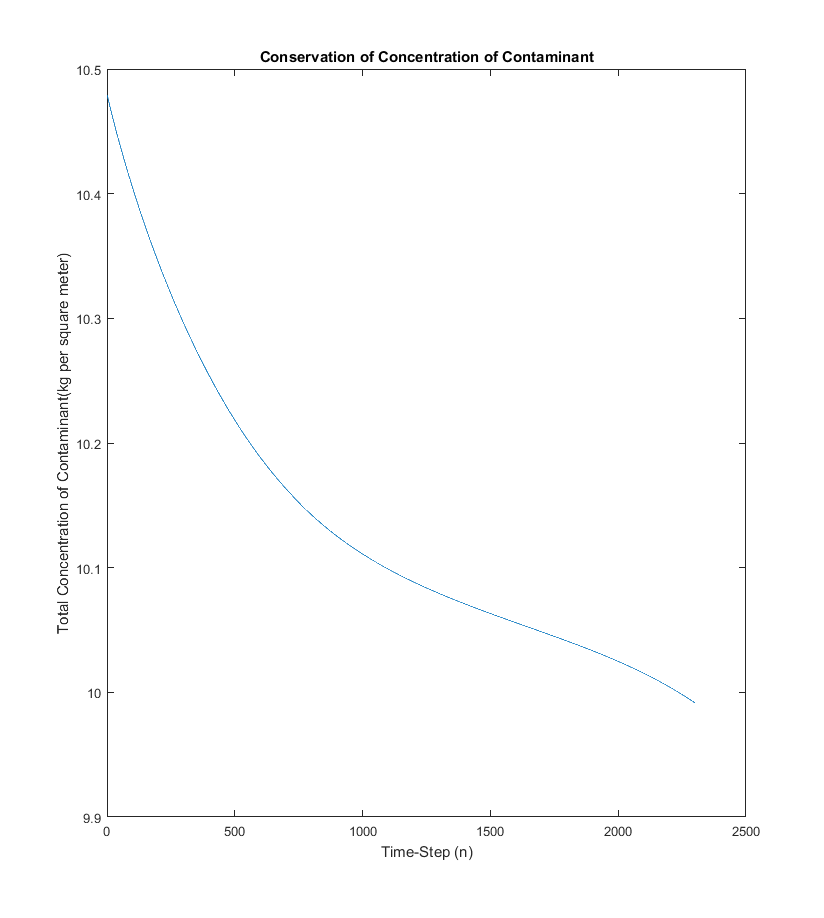
\includegraphics[trim=0mm 0mm 0mm 0mm,clip,width=1.11\linewidth]{pointconservation.png}
%\caption{Conservation of Concentration of Contaminant}
\end{minipage}
 \begin{minipage}[b]{0.496\textwidth}
   \includegraphics[trim=0mm 0mm 0mm 0mm,clip,width=1.11\linewidth]{derivpointconservation.png}
%\caption{Deriviative of Concentration of Contaminant}
\end{minipage}
\end{figure}
\hyperlink{Questions}{\beamergotobutton{Questions}}
\end{frame}

\begin{frame}{Increase in Concentration of Contaminant for Constant Source Model}\label{ConstIncrease}

\begin{itemize}
\item Test for linear increase in concentration of contaminant in constant source model
\end{itemize}

\begin{figure} 
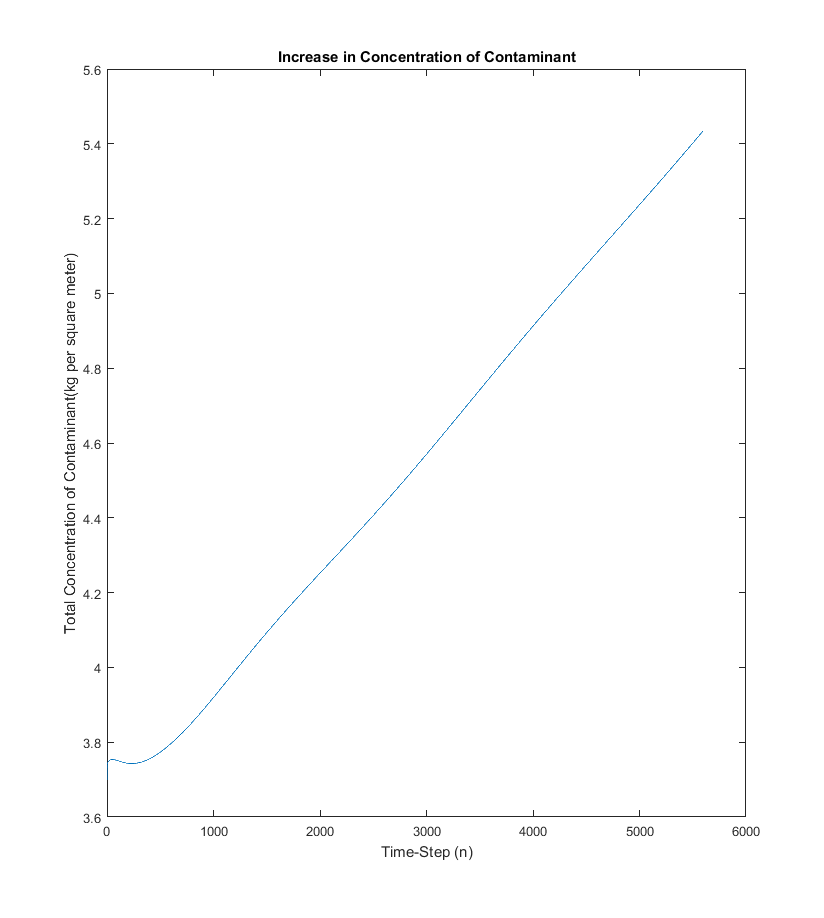
\includegraphics[trim=0mm 0mm 0mm 0mm,clip,width=.61\linewidth]{constincrease.png}
\end{figure}
\hyperlink{Questions}{\beamergotobutton{Questions}}
\end{frame}

\section{Sensitivity Analyses}

\begin{frame}{Domain Region used for Sensitivity}\label{Region}

\begin{itemize}
\item Measure contaminant flow through the region shown
\end{itemize}

\begin{figure} 
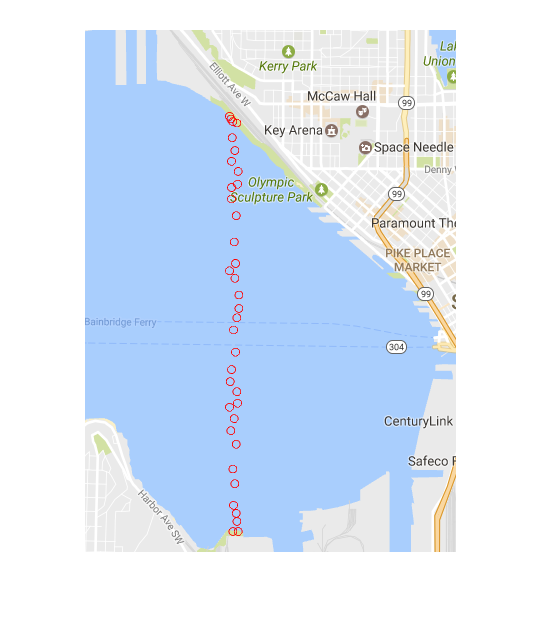
\includegraphics[trim=0mm 0mm 0mm 0mm,clip,width=0.5\linewidth]{sensewall.png}
\end{figure}
\hyperlink{Questions}{\beamergotobutton{Questions}}
\end{frame}

\begin{frame}{Graphical Sensitivity} \label{Graphical Sensitivity}

\begin{figure}   
\begin{minipage}[b]{0.496\textwidth}
   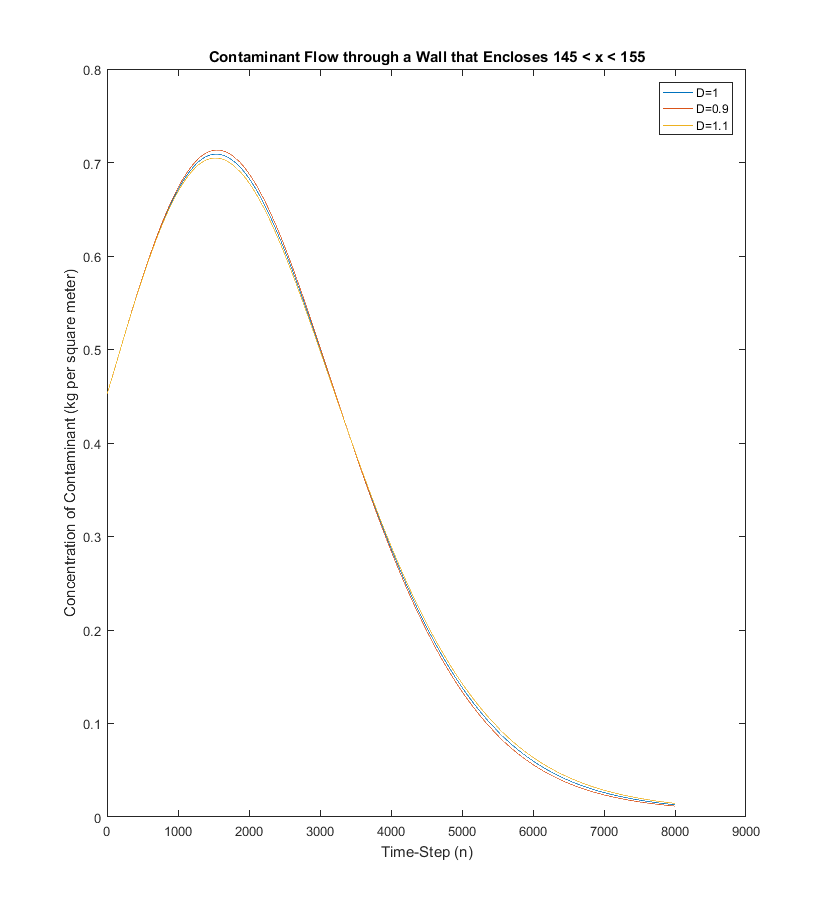
\includegraphics[trim=0mm 0mm 0mm 0mm,clip,width=1.1\linewidth]{sensepoint.png}
\begin{center}
%\caption{Point Source Model Sensitivity}
\end{center}
\end{minipage}
 \begin{minipage}[b]{0.496\textwidth}
   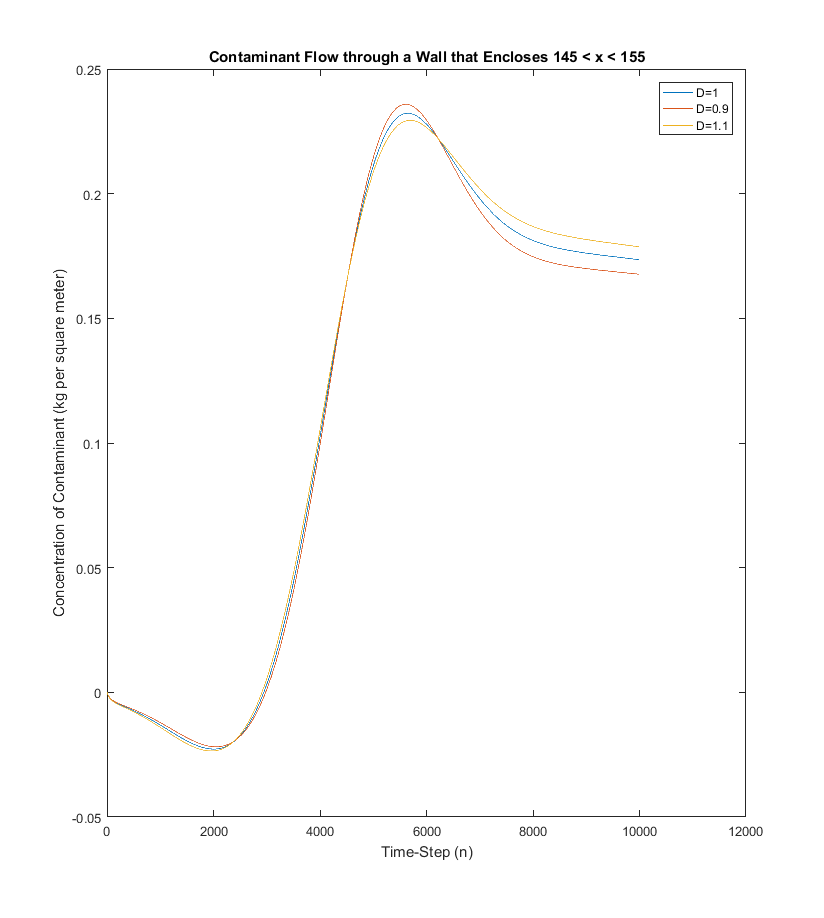
\includegraphics[trim=0mm 0mm 0mm 0mm,clip,width=1.1\linewidth]{senseconst.png}
\begin{center}
%\caption{Constant Source Model Sensitivity}
\end{center}
\end{minipage}
\end{figure}
\hyperlink{Questions}{\beamergotobutton{Questions}}
\end{frame}

\begin{frame}{Sensitivity at a Time Step}\label{Sensitivity at time step}

\begin{table}
\caption{Sensitivity Point Source Model at $n=1900$}
\begin{tabular}{|l|l|}
\hline
Change in Diffusivity $D$          & $S$ \\ \hline
$+10\%$    & $-0.0773$              \\ \hline
$-10\%$   & $0.0646$              \\ \hline
\end{tabular}
\end{table}

\begin{table}
\centering
\caption{Sensitivity Constant Source Model at $n=5900$}
\begin{tabular}{|l|l|}
\hline
Change in Diffusivity $D$           & $S$ \\ \hline
$+10\%$    & $-0.0893$              \\ \hline
$-10\%$   & $0.0870$              \\ \hline
\end{tabular}
\end{table}
\hyperlink{Questions}{\beamergotobutton{Questions}}
\end{frame}

\section{Conclusion}

\begin{frame}{Future Work} \label{FW}
\begin{itemize}
\item Use optimized meshing code
\item Avoid using a barycentric approximation of the basis functions
\item Use a realistic diffusivity and magnitude of velocity
\item Refine tolerance scheme used to connect finite element code and finite difference code
\end{itemize}

\hyperlink{Questions}{\beamergotobutton{Questions}}
\end{frame}

\begin{frame}{Thank you}
    \begin{center}
        {\bf Thank you!}
    \end{center}
\end{frame}

\begin{frame}{Questions}\label{Questions}
    %\begin{center}
        %{\bf Questions?}
\begin{itemize}
\item \hyperlink{Purpose}{\beamergotobutton{Purpose}}
\item \hyperlink{Puget Sound Domain}{\beamergotobutton{Puget Sound Domain}}
%\item \hyperlink{Puget Sound Domain Triangularization}{\beamergotobutton{Puget Sound Domain Triangularization}}
\item\hyperlink{The Advection-Diffusion Equation}{\beamergotobutton{The Advection-Diffusion Equation}}
\item \hyperlink{EulerandWeak}{\beamergotobutton{Implict Euler Step and the Weak Form}}
\item\hyperlink{basisfunctionandfinite}{\beamergotobutton{Creation of Basis Functions and Finite Element Discretization}}
\item\hyperlink{applyingFEMtoweakform}{\beamergotobutton{Applying the Finite Element Discretizations to the Weak Form}}
\item\hyperlink{BuildLinearSystem}{\beamergotobutton{Building the Linear System}}
\item\hyperlink{MassmatRHSLinearSystem}{\beamergotobutton{Mass Matrices, Right-Hand Side, and the Linear System}}
\item\hyperlink{ComputationofC}{\beamergotobutton{Computation of $\mathbf{C}$}}
\item\hyperlink{NavierStokesSlide}{\beamergotobutton{Implementation of the Navier-Stokes Equations}}
\item\hyperlink{NavierStokesSteadyState}{\beamergotobutton{Steady State Solution to the Navier-Stokes Equations}}
\item\hyperlink{PointSourceModelResults}{\beamergotobutton{Point Source Model}}
\item\hyperlink{ConstantSourceModelResults}{\beamergotobutton{Constant Source Model}}
\item\hyperlink{ConvergenceTesting}{\beamergotobutton{Convergence Testing}}
\item\hyperlink{PointConservation}{\beamergotobutton{Conservation of Concentration of Contaminant for Point Source Model}}
\item\hyperlink{ConstIncrease}{\beamergotobutton{Increase in Concentration of Contaminant for Constant Source Model}}
\item\hyperlink{Region}{\beamergotobutton{Domain Region used for Sensitivity}}
\item\hyperlink{Graphical Sensitivity}{\beamergotobutton{Graphical Sensitivity}}
\item\hyperlink{Sensitivity at time step}{\beamergotobutton{Sensitivity at a Time Step}}
\item\hyperlink{FW}{\beamergotobutton{Future Work}}

\end{itemize}
    %\end{center}
\end{frame}

\begin{frame}{Works Cited}
\begin{thebibliography}{4}
\bibitem{50LinesofMATLAB}
\textit{Remarks around 50 lines of Matlab: short finite element implementation}, Jochen Alberty, Carsten Carstensen and Stefan A. Funken, \textit{Numerical Algorithms 20} (1999), pp. 117-137

\bibitem{Johnson}
\textit{Numerical Solution of Partial Differential Equations by the Finite Element Method}, Claes Johnson, Dover Publications, INC. Mineola, New York (2009) pp. 14-20

%\bibitem{DiffusivityCoefficientat22degrees}
%\textit{Modeling the BP Oil Spill of 2010: A Simplified Model of Oil Diffusion in Water}, Eilleen Ao-leong, Anna Chang, Steven Gu, \textit{BENG 221 - Fall 2012} (2012) pp. 4

%\bibitem{Kinematic Viscosity of Water at 22 degrees}
%http://www.viscopedia.com/viscosity-tables/substances/water/

\bibitem{Sullivan}
Dr. Eric Sullivan, Assistant Professor of Mathematics, Carroll College (2017)

\end{thebibliography}
\end{frame}

\end{document}






    





       